

%The proton PDFs are classically extracted from QCD fits by a measure of 
%the agreement between experimental data and corresponding theory models.
%During the fit procedure in the \fitter\ framework, the PDFs are
%parametrised at a starting scale $Q^2_0$ chosen to be below the charm 
%mass threshold and then evolved using coupled, integro-differential
%Dokshitzer-Gribov-Lipatov-Altarelli-Parisi 
%(DGLAP)~\cite{Gribov:1972ri,Gribov:1972rt,Lipatov:1974qm,
%Dokshitzer:1977sg,Altarelli:1977zs} evolution equations 
%as implemented in the QCDNUM~\cite{qcdnum} program in the $\overline{\text{MS}}$ scheme. 
%The evolution can be performed in the LO, NLO or NNLO accuracy~\cite{Curci:1980uw,Furmanski:1980cm}.
%
In this section the theoretical formalism based on DGLAP \cite{Gribov:1972ri,Gribov:1972rt,Lipatov:1974qm,Dokshitzer:1977sg,Altarelli:1977zs} equations
% equations for various processes 
%available in \fitter 
is described. 

A direct consequence of factorisation (Eq. \ref{eq:fact}) is that the scale dependence or ``evolution'' of the PDFs can be predicted 
by the renormalisation group equations. 
By requiring physical observables to be independent of 
$\muf$, a representation 
of the parton evolution in terms of the DGLAP equations is obtained:
%integro-differential equations known as 
%DGLAP~\cite{Gribov:1972ri,Gribov:1972rt,Lipatov:1974qm,Dokshitzer:1977sg,Altarelli:1977zs} (Dokshitzer-Gribov-Lipatov-Altarelli-Parisi) equations:

\begin{eqnarray}
%\frac{d~f_i(x,\mur,\muf)}{d \log\muf^2} = \sum_{j=q\bar{q},g}\int_{x}^{1}\frac{d y}{y} 
%P_{ij}\left(\frac{x}{y};\alpha_s,\mur,\muf\right) f_j(y,\mur,\muf)\,,
\frac{d~f_a(x,\muf^2)}{d \log\muf^2} = \sum_{b=q,\bar{q},g}\int_{x}^{1}\frac{d z}{z} 
P_{ab}\left(\frac{x}{z};\muf^2\right) f_b(z,\muf^2)\,,
\label{eq:dglap}
\end{eqnarray}
%
where the functions $P_{ab}$ are the evolution kernels or splitting functions, which represent the probability 
of finding parton $a$ in parton $b$. They can be calculated as a  perturbative expansion in $\alpha_s$. 
%The analytic structure of $P_{ij}$ is known at 3-loop in perturbation theory and can be found in the literature. 
Once PDFs are determined at the initial
scale $\mu_F^2 = Q_0^2$, their evolution to any other scale $Q^2 > Q_0^2$ is entirely determined by the DGLAP equations.
The PDFs are then used to calculate cross sections for various different processes.
Alternative approaches to DGLAP evolution equations, valid in different kinematic regimes, 
are also implemented in \fitter and will be discussed in Sec.~\ref{sec:alternative}.


%The PDFs are determined by measuring the agreement 
%the agreement between experimental data and corresponding theory models within 
%the DGLAP~\cite{Gribov:1972ri,Gribov:1972rt,Lipatov:1974qm,
%Dokshitzer:1977sg,Altarelli:1977zs} formalism.
%Models which are available in \fitter\ for various processes are described in the following text.



\subsection{Deep Inelastic Scattering and Proton Structure}
\label{dissection}


%DIS data provide the backbone of any PDF fit.
The for\-ma\-lism that relates the DIS measurements to pQCD and the PDFs has been described
in detail in many extensive reviews (see e.g. Ref. \cite{disbook}) and it is only briefly summarised here.
DIS is the process where a lepton scatters off the partons in the proton
by the virtual exchange of a neutral ($\gamma/Z$) or charged ($W^{\pm}$) vector boson and, as a result, a scattered lepton and a 
hadronic final state are produced.
The common DIS kinematic variables are the scale of the process $Q^2$, which is the absolute squared four-momentum of 
the exchanged boson, Bjorken $x$, 
which can be related in the parton model to 
the momentum fraction that is carried by the struck quark, 
and the inelasticity $y$. These are related by $y=Q^2/sx$, where $s$ is the squared centre-of-mass energy.
%$s = 4E_eE_p$ at HERA.
%which is the fraction of the energy 
%transferred to the hadronic vertex.
\\
%
The NC cross section can be expressed in terms of generalised structure functions:
\begin{eqnarray}
%  \nonumber
    \frac{d^2\sigma_{NC}^{e^{\pm} p}}{dxdQ^2}&=&\frac{2\pi\alpha^2 Y_{+}}{xQ^4} \sigma_{r,NC}^{e^{\pm} p},\\ 
    \sigma_{r,NC}^{e^{\pm} p}&= &  \tilde F_2^{\pm} \mp \frac{Y_{-}}{Y_{+}}x \tilde F_3^{\pm} - \frac{y^2}{Y_{+}} \tilde F_L^{\pm},
 %\label{eq:NC not reduced}
\end{eqnarray}
where  $Y_{\pm} = 1 \pm (1-y)^2$ and $\alpha$ is the electromagnetic coupling constant.
%the photon propagator and a helicity factor are factored out in the definition of the reduced cross section $\sigma_r$.
%, and  $Y_{\pm} = 1 \pm (1-y)^2$ (additional terms of $O(1/Q^2)$ are numerically sm%all 
%at the HERA kinematics and are neglected). 
The generalised structure functions $\tilde F_{2,3}$ 
can be written as linear combinations of the proton structure functions $F^{\gamma}_2, F^{\gamma Z}_{2,3}$ 
and $F^Z_{2,3}$, which are associated with pure photon exchange terms, photon-$Z$ interference
terms and pure $Z$ exchange terms, respectively. 
The structure function $\tilde F_2$ is the dominant contribution to the cross section, 
$x \tilde F_3$ becomes important at high $Q^2$ and $\tilde F_L$ is sizable 
only at high $y$. 
In the framework of pQCD, the structure functions are directly related to the 
PDFs: at LO $F_2$ is the weighted momentum sum of quark and anti-quark distributions, 
%$F_2 \approx x \sum e^2_q (q+ \overline q)$
 $xF_3$ is related to their difference, 
%$xF_3 \approx x \sum 2e_q a_q (q- \overline q)$ (where $a_q$ is the axial-vector 
%quark coupling and $e_q$ the quark electric charge)
and $F_L$ vanishes. At higher orders, terms related to the gluon distribution
appear, in particular $F_L$ is strongly related to the low-$x$ 
gluon.
\\
The inclusive CC $ep$ cross section, analogous to the NC $ep$ case, can be expressed in terms of another set 
of structure functions, $\tilde W$: 
\begin{eqnarray}
\centering
%  \nonumber
%    \begin{array}{rll}
   \frac{d^2\sigma_{CC}^{e^{\pm} p}}{dxdQ^2}&=&\frac{1\pm P}{2}\frac{G^2_F}{2\pi x}\big [\frac{m^2_W}{m^2_W+Q^2}\big ]\sigma_{r,CC}^{e^{\pm} p}\\
   \sigma_{r,CC}^{e^{\pm} p}&= &  Y_{+} \tilde W_2^{\pm} \mp Y_{-}x \tilde W_3^{\pm} - y^2 \tilde W_L^{\pm},
%      \sigma_{r,CC}^{e^{+} p} &\approx& 
%        x [\overline u + \overline c] + (1-y)^2 x [d+s], \\
%      \sigma_{r,CC}^{e^{-} p} &\approx& 
%        x[u+c] + (1-y)^2 x[\overline d + \overline s],
%    \end{array}
\end{eqnarray}
where $P$ represents the lepton beam polarisation.
% and $\tilde W_2$, $\tilde W_3$,$\tilde W_L$ are structure functions.
At LO in $\alpha_s$, the CC $e^+p$ and $e^-p$ cross sections are sensitive to 
different combinations of the quark flavour densities.
% \begin{eqnarray}
%     \sigma_{r,CC}^{e^{+} p} &\approx& 
%       x [\overline u + \overline c] + (1-y)^2 x [d+s], \\
%     \sigma_{r,CC}^{e^{-} p} &\approx& 
%       x[u+c] + (1-y)^2 x[\overline d + \overline s],
% \end{eqnarray}
%Here $U$ and $D$ denote the sum over up- and down-type quarks;
%the latter include also strange and beauty quarks and 
%the former charm quarks.

Beyond LO, the QCD predictions for the DIS structure functions are obtained by convoluting 
the PDFs with appropriate hard-process scattering matrix elements, which are referred to as coefficient functions. 


%Here $U$ and $D$ denote the sum over up- and down-type quarks;
%the latter include also strange and beauty quarks and 
%the former charm quarks.
%
%Beyond LO, 
%{\bf check this sentence if it makes sense}.
%The QCD predictions for the DIS structure functions are obtained by convoluting 
%the PDFs with the respective coefficient functions. 

The DIS measurements span a large range of $Q^2$ from a few $\GeV^2$ to about $10^5$ $\GeV^2$, crossing heavy quark mass thresholds, thus the treatment of heavy quark (charm and beauty) 
production and the chosen values of their masses become important. 
There are different schemes for the treatment of heavy quark production. 
%that would be equivalent if calculations could be carried out to all orders in $\alpha_s$, but which differ at finite order.
Several variants of these schemes are implemented in \fitter and they are briefly discussed below.
%\begin{description}

\paragraph{Zero-Mass Variable Flavour Number (ZM-VFN)\rm:\\}
In this scheme~\cite{ZMVFNpub}, the
heavy quarks appear as partons in the proton at $Q^2$ values above $\sim m_h^2$ (heavy quark mass)
and they
%for $Q^2>>m_h^2$ but 
are then treated as massless in both the initial 
and final states of the hard scattering process. The lowest order process is the
%scattering of a heavy quark in the proton with the lepton via (electroweak) boson exchange.
scattering of the lepton off the heavy quark via electroweak boson exchange.
This scheme is expected to be reliable in the region where $Q^2 \gg m_h^2$.
%This is the scheme that had been used in the past by PDF groups.
In \fitter this scheme is available for the DIS structure function calculation 
via the interface to the \qcdnum \cite{qcdnum} package, thus it benefits 
from the fast \qcdnum convolution engine.

\paragraph{Fixed Flavour Number (FFN)\rm:\\} 
In this rigorous quantum field theory scheme \cite{Laenen:1992, Laenen:1993, Riem:1995}, 
only the gluon and the light quarks are considered
as partons within the proton and massive 
quarks are produced perturbatively in the final state.
The lowest order process is
the heavy quark-antiquark pair production via boson-gluon fusion.
%the fusion of a gluon in the proton
%with a boson from the lepton to produce a heavy quark and an antiquark.
%The recent series of PDFs that use this scheme as default are ABM and JR PDF groups.
In \texttt{HERA}\texttt{Fitter} this scheme can be accessed via the 
\qcdnum implementation or through the interface to the open-source code \texttt{OPENQCDRAD}~\cite{openqcdrad:page} as implemented by the ABM group.
This scheme is reliable for $Q^2 \sim m_h^2$.
In \qcdnum, the calculation of the heavy quark contributions to DIS structure functions
are available at Next-to-Leading Order (NLO) and only electromagnetic exchange contributions are taken into account. 
In the \texttt{OPEN}\texttt{QCDRAD} implementation the heavy quark contributions to CC structure functions are also available 
%and, for the NC case, the QCD corrections to the massive Wilson coefficients at Next-to-Next-to Leading Order (NNLO)
and, for the NC case, the QCD corrections to the coefficient functions in Next-to-Next-to Leading Order (NNLO)
are provided in the best currently known approximation~\cite{SMoch:npb864,Bierenbaum:2009mv}.
The  \texttt{OPENQCDRAD} implementation uses in addition the running heavy quark mass in the $\overline{\text{MS}}$ scheme~\cite{Alekhin:runm}.

It is sometimes argued that this scheme reduces the sensitivity of the DIS cross sections to higher order 
corrections ~\cite{SMoch:npb864,Bierenbaum:2009mv}. It is also known to have smaller non-perturbative corrections than the pole mass scheme 
\cite{Beneke:1998ui}.

\paragraph{General-Mass Variable Flavour Number (GM-VFN)\rm:\\}
In this scheme \cite{VFN}, heavy quark production is treated for
$Q^2 \sim m_h^2$ in the FFN scheme and for $Q^2 \gg m_h^2$
in the massless scheme with a suitable interpolation in between. 
The details of this interpolation differ between implementations.
%in the ZM-VFN scheme with a suitable interpolation in between.
The groups that use GM-VFN schemes in PDFs are MSTW, CT (CTEQ), NNPDF, and HERAPDF.
%This scheme is very popular and numerous variants exist.
\fitter implements different variants of the GM-VFN scheme.
% 
\begin{itemize}
%
\item \it {GM-VFN Thorne-Roberts scheme:} \rm
%\subsubsection{GM-VFN Thorne-Roberts scheme}
%
%The Thorne-Roberts (TR) scheme provides a smooth transition from the massive FFN
%scheme at low scales $Q^2<m_h^2$ to the massless ZM-VFNS scheme at  
%high scales $Q^2>>m_h^2$.
%There are two different variants of the TR schemes: TR standard 
%(as used in MSTW PDF 
%sets~\cite{Thorne:1997ga,Thorne:2006qt,MSTWpdf}) 
%and TR optimal~\cite{Thorne:6180}, with a smoother transition across the heavy quark threshold region.
%Both of these variants are accessible within the \fitter package at 
%NLO and NNLO.  
%
The Thorne-Roberts (TR) scheme~\cite{Thorne:1997ga} was designed to provide a smooth transition 
from the massive FFN scheme at low scales $Q^2 \sim m_h^2$ to the massless ZM-VFNS scheme at high scales $Q^2 \gg m_h^2$. 
Because the original version was technically difficult to implement beyond NLO, it was updated 
to the TR$^\prime$ scheme~\cite{Thorne:2006qt}.
%which is simpler (and closer to the ACOT-scheme, see below).
There are two variants of the TR$^\prime$ schemes: TR$^\prime$ standard (as used in MSTW PDF sets~\cite{Thorne:2006qt,MSTWpdf}) 
and TR$^\prime$ optimal~\cite{Thorne:6180}, with a smoother transition across the heavy quark threshold region. 
Both TR$^\prime$ variants are accessible within the \fitter package at LO, NLO and NNLO.
%%%%
\vspace{0.1cm}
\item \it {GM-VFN ACOT scheme:} \rm
The Aivazis-Collins-Olness-Tung (ACOT) scheme belongs to the group of VFN factorisation 
schemes that use the renormalisation method of Collins-Wilczek-Zee (CWZ) \cite{CWZ}.
This scheme unifies the low scale $Q^2 \sim m_h^2$ and high scale $Q^2 > m_h^2$ regions
%with a smooth interpolation across the full energy range. 
in a coherent framework across the full energy range.
%
Within the ACOT package, the following variants of the ACOT $\overline{\text{MS}}$ scheme are available at LO and NLO:
ACOT-Full \cite{Aivazis:1993pi}, S-ACOT-$\chi$ \cite{Kramer:2000hn,Kretzer:2003it} and ACOT-ZM \cite{Aivazis:1993pi}.
For the longitudinal structure function higher order calculations are also available. 
A comparison of PDFs extracted from QCD fits to the HERA data 
with the TR$^\prime$ and ACOT-Full schemes is illustrated in Fig.~\ref{fig:acotrt} (taken from \cite{h1zeus:2009wt}).

\begin{figure}[!ht]
\centering
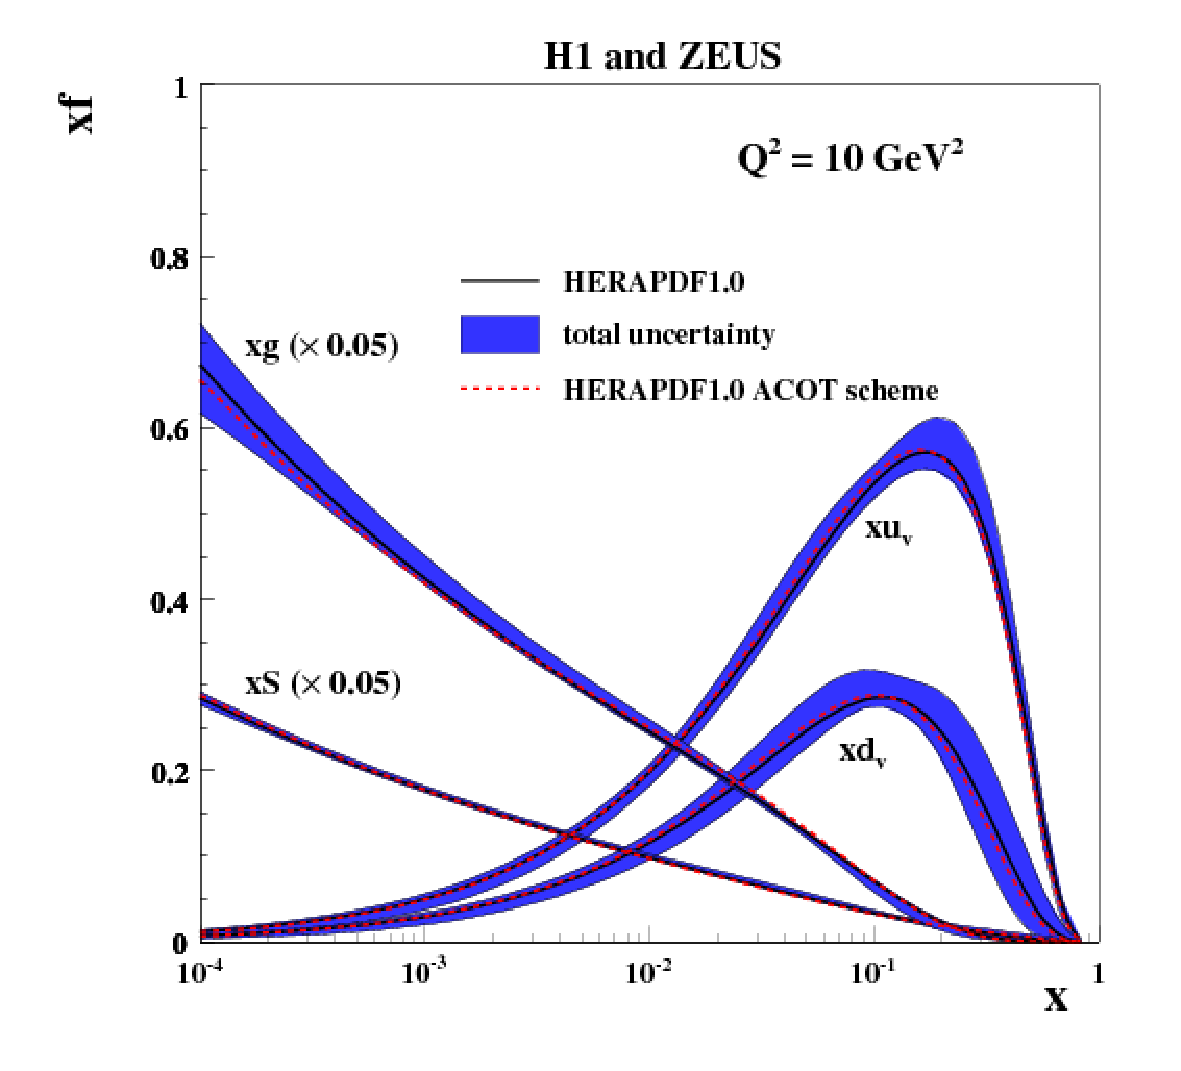
\includegraphics[width=8cm]{heraacot}
   \caption{Distributions of valence ($xu_v$, $xd_v$), sea ($xS$) and the gluon ($xg$) PDFs in HERAPDF1.0~\cite{h1zeus:2009wt}
       with their total uncertainties at the scale of $Q^2 = 10\ \GeV^2$ obtained 
       using the TR$^\prime$ scheme and compared to the PDFs obtained with 
       the ACOT-Full scheme using the $k$-factor technique (red).
       The gluon and the sea distributions are scaled down by a factor of 20.}
 \label{fig:acotrt}
\end{figure}


%\vspace{0.1cm}
\end{itemize}
%\end{description}

\subsection{Electroweak Corrections to DIS}
%%%%%%%%%%%
%\item \bf {Electroweak corrections for \texorpdfstring{$ep$}{ep} scattering:} \rm
Calculations of higher-order electroweak corrections to DIS at 
HERA are available in \fitter in the on-shell scheme. In this scheme, the
masses of the gauge bosons $m_W$ and 
$m_Z$ are treated as basic parameters together with the top, 
Higgs and fermion masses.
These electroweak corrections 
are based on the \texttt{EPRC} package~\cite{SpiesbergerPrivComm}.
The code calculates the running of the electromagnetic coupling $\alpha$ using the most recent parametrisation
of the hadronic contribution
% to $\Delta_\alpha$ 
\cite{Jegerlehner} as well as 
an older version from Burkhard \cite{Burkhard}.



\subsection{Diffractive PDFs}

\newcommand{\asotp}{\ensuremath{\frac{\alpha_{\rm s}}{2\pi}}}
\newcommand{\Sgl}[1]{\ensuremath{\tilde f_{#1+}}}
\newcommand{\Pom}{{I\!P}}
\newcommand{\Reg}{{I\!R}}
\newcommand{\xpom}{$x_{I\!P}$}
\newcommand{\xP}{x_\Pom}


%Similarly to standard PDFs,
About 10\% of deep inelastic interactions at HERA are diffractive, such that the interacting proton stays intact ($ep\to eXp$). 
The outgoing proton is separated from the rest of the final hadronic system, $X$, by a large rapidity gap.  
Such events are a subset of DIS where the hadronic state $X$ comes from the interaction of the
virtual photon with a colour-neutral cluster stripped off the proton \cite{Hebecker:1999vf}.
The process can be described analogously to the inclusive DIS, by means of the diffractive parton distributions 
(DPDFs) \cite{Collins:1997sr}.
The parametrization of the colour-neutral exchange in terms of factorisable `hard' Pomeron and a secondary 
Reggeon \cite{Ingelman:1984ns}, both having a hadron-like partonic structure, 
has proved remarkably successful in the description of most of the diffractive data.
It has also provided a practical method to determine DPDFs from fits to the diffractive cross sections.
%The proton is well separated from the 
%rest of the hadronic final state by a large rapidity gap.  
%This is interpreted as the dissociation of the virtual photon into a
%hadronic system $X$ with a squared invariant mass much 
%smaller than the photon-proton centre-of-mass energy $W^2=ys-Q^2+m_p^2(1-y)$, where $m_p$ is the proton mass. 
%Such a process is often assumed to be mediated by the exchange of a hard Pomeron 
%or a secondary Reggeon with vacuum quantum numbers. 
%This factorisable Pomeron picture has proved remarkably successful in the description of most of the diffractive data.
%Diffractive parton distributions (DPDFs) 
%can be determined from QCD fits to diffractive cross sections in a similar way to the determination of the standard PDFs \cite{Collins:1997sr}.

%
%\begin{figure}[!ht]
%\begin{center}
%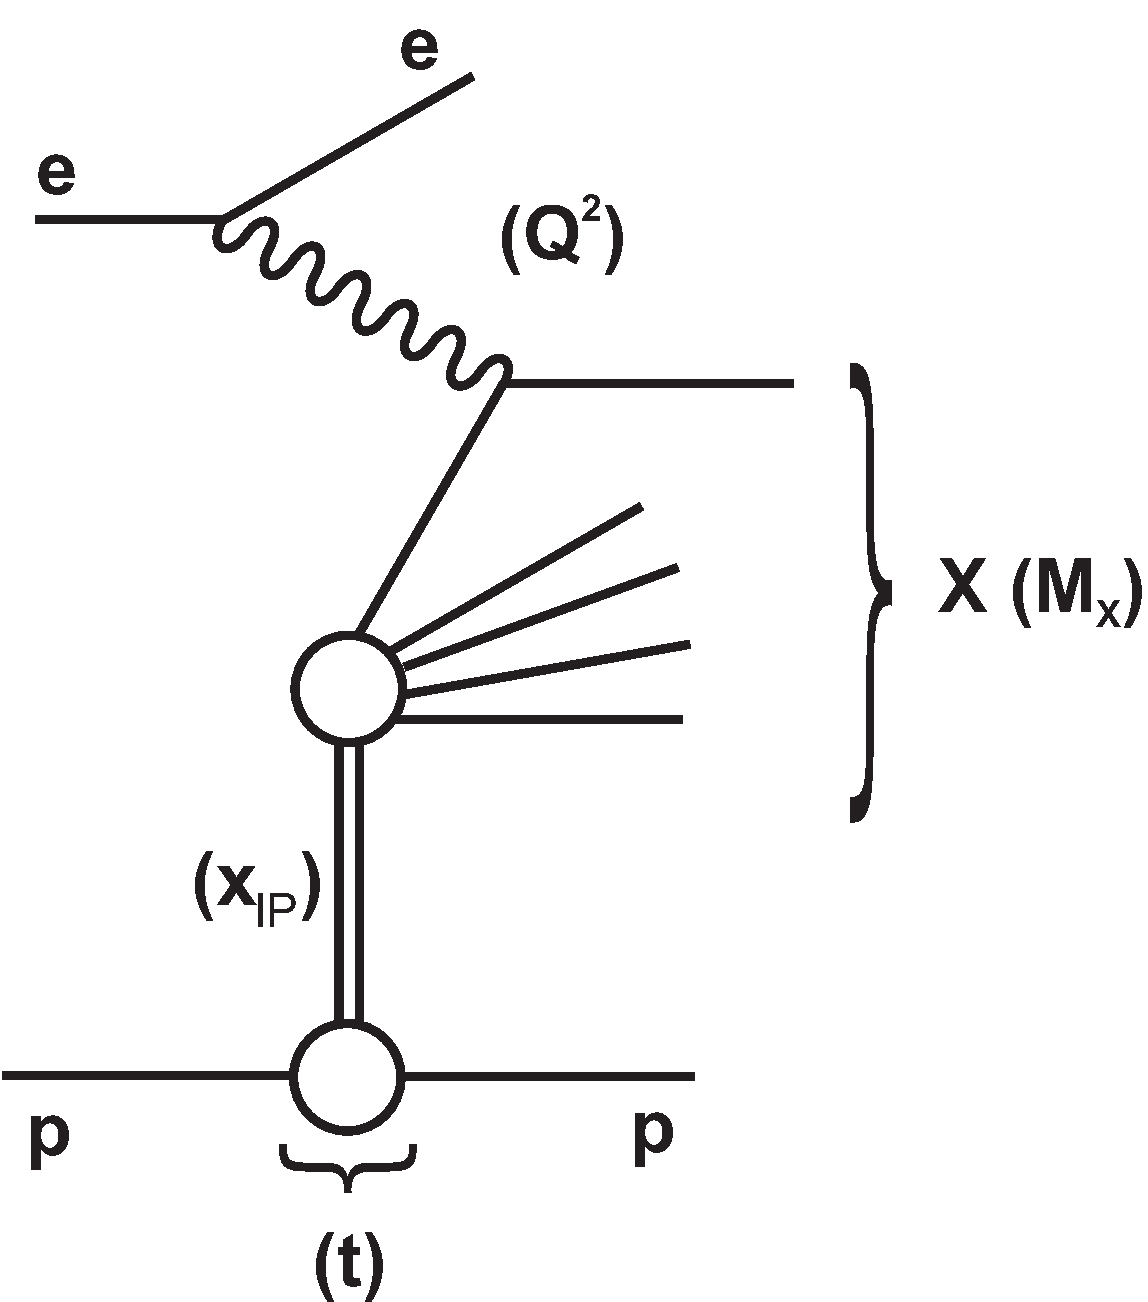
\includegraphics[width=0.5\linewidth]{figures/diffraction.pdf}
%\end{center}
%\caption{Schematic diagram of the kinematic variables used to
% describe the inclusive diffractive DIS process.}
%\label{fig:diff}
%\end{figure}

In addition to the usual DIS variables $x$, $Q^2$, extra kinematic variables are needed to describe the diffractive process. 
These are the squared four-momentum transfer of the exchanged Pomeron or Reggeon, $t$, and 
%(the undetected momentum transfer to the proton system) and
the mass $m_X$ of the diffractively produced final state. 
In practice, the variable $m_X$ 
is often replaced by the dimensionless quantity $\beta=\frac{Q^2}{m_X^2+Q^2-t}$.
In models based on a factorisable Pomeron, $\beta$ may be viewed at LO as the fraction of the
Pomeron longitudinal momentum, $x_{\Pom}$, which is carried by the struck parton, $x=\beta x_{\Pom}$,
where $P$ denotes the momentum of the proton.
%The diffractive parton distribution functions (DPDFs) are interpreted as probabilities for 
%finding a parton with a small fraction of the proton momentum $x=\beta\Pom$
\\
For the inclusive case, the diffractive cross section reads as:
\begin{equation}
\begin{array}{lcl}
    \frac{d^4\sigma}{d\beta\,dQ^2dx_{\Pom}\,dt}
=
  \frac{2\pi\alpha^2}{\beta Q^4}\,
    \left( 1 +  (1-y)^2 \right) \ensuremath{\overline\sigma}^{D(4)}(\beta,Q^2,x_{\Pom},t)
\label{Dxs}
\end{array}
\end{equation}
with the ``reduced cross section'': 
\begin{equation}
\begin{array}{lcl}
\overline\sigma^{D(4)}
 = F_2^{D(4)} - \frac{y^2}{1 +  (1-y)^2}\, F_L^{D(4)}.
% = F_T^{D(4)} + \frac{2(1-y)}{1 +  (1-y)^2}\, F_L^{D(4)}.
\label{eq:sigred}
\end{array}
\end{equation}
%The dimension of $F_k^{D(4)}(\beta,Q^2,x_{\Pom},t)$
%is $GeV^{-2}$ and thus quantities integrated over $t$.
%\begin{equation}
%F_k^{D(3)}(\beta,Q^2,x_{\Pom})
%\equiv
%\int_{t_{\rm min}}^{t_{\rm max}} dt
%F_k^{D(4)}(\beta,Q^2,x_{\Pom},t)
%\end{equation}
%are dimensionless. The maximum kinematically allowed value of $t$ is given by
%\begin{equation}
%t_{\rm MAX} 
%=
%-\frac{x_{\Pom}^2 m_p^2 + p_\perp^2}{1-x_{\Pom}}
%\approx 
%-\frac{x_{\Pom}^2}{1-x_{\Pom}} m_p^2
%\end{equation}
%where $m_p$ is the proton mass.

%Substituting $x = x_{\Pom}\beta$ we can relate Eq.~\ref{Dxs} to the standard DIS formula.
%\begin{equation}
%\begin{array}{lcl}
%\frac{d\sigma}{d\beta\,dQ^2\,dx_{\Pom}\,dt} =
%  \frac{2\pi\alpha^2}{x\, Q^4}\,
%    \left( 1 +  (1-y)^2 \right) x_{\Pom}\ensuremath{\overline\sigma}^{D(4)}(\beta,Q^2,x_{\Pom},t)
%\end{array}
%\end{equation}
%which upon integration over $t$ reads
%\begin{equation}
%\begin{array}{lcl}
%\label{Dxs3}
%  \frac{d\sigma}{d\beta\,dQ^2\,dx_{\Pom}}
%=  
%  \frac{2\pi\alpha^2}{x Q^4}\,
%    \left( 1 +  (1-y)^2 \right) \,x_{\Pom}\ensuremath{\overline\sigma}^{D(3)}(\beta,Q^2,x_{\Pom}).
%\end{array}
%\end{equation}
%%The H1 and ZEUS data files typically contain $x_{\Pom}\ensuremath{\overline\sigma}^{D(3)}$.
The diffractive structure functions can be expressed as convolutions of 
calculable coefficient functions with the diffractive quark and gluon distribution functions,
 which in general depend on \xpom, $Q^2$, $\beta$ and $t$.

The DPDFs \cite{Aktas:2006hy, zeus:diff2009} in \fitter are implemented as a sum 
of two factorised contributions:
\begin{equation}
 \Phi_\Pom(\xP,t)\, f^{\Pom}_{a}(\beta,Q^2)
  + 
 \Phi_\Reg(\xP,t)\, f^{\Reg}_{a}(\beta,Q^2)
 \,,
\end{equation} 
where $\Phi(\xP,t)$ are the Reggeon and Pomeron fluxes.
The Reggeon PDFs, $f^{\Reg}_{a}$ are fixed as those of the pion, while the Pomeron PDFs,
$f^{\Pom}_{a}$, can be obtained from a fit to the data.

%==========================================
%{\bf Regge factorization} 
%Needed? \\
% The diffractive PDFs in \fitter\ are implemented following the prescription of ZEUS
% collaboration \cite{zeus:diff2009}.
%and can be used to reproduce their results.
%For a  better description of data, a contribution from a secondary Reggeon, $\Reg$, is included, hence
%\begin{equation}
%F_k^{D(4)}(\beta,Q^2,x_{\Pom},t) = 
%\sum_{\mathcal{X} =\Pom,\Reg}
%\phi_\mathcal{X}(x_{\Pom},t)\, F^\mathcal{X}_k(\beta,Q^2)
%\end{equation}
%or
%\begin{equation}
%\label{eq:FD3}
%F_k^{D(3)}(\beta,Q^2,x_{\Pom}) = 
%\sum_{\mathcal{X} =\Pom,\Reg}
%\Phi_\mathcal{X}(x_{\Pom})\, F^\mathcal{X}_k(\beta,Q^2)
%\end{equation}
%where
%\begin{equation}
%\label{eq:intFlux}
%\Phi_{\mathcal{X}}(x_{\Pom}) =
%\int\limits_{t_{\rm min}}^{t_{\rm max}} dt\, \phi_\mathcal{X}(x_{\Pom},t)
%\,.
%\end{equation}
%The fluxes are parametrized as
%\begin{subequations}
%\label{eq:flux}
%\begin{equation}
%\phi_\mathcal{X}(x_{\Pom},t) = 
%\frac {A_\mathcal{X}\, e^{b_\mathcal{X} t}} {x_{\Pom}^{2\alpha_\mathcal{X}(t) -1}}
%\end{equation}
%where
%\begin{equation}
%\alpha_\mathcal{X}(t) = \alpha_\mathcal{X}(0) + \alpha_\mathcal{X}' t
%\,.
%\end{equation}
%\end{subequations}
%The function $F^\Reg_k(\beta,Q^2)$  is taken to be that of the pion.
%




\subsection{Drell-Yan Processes in $pp$ or $p\bar p$ Collisions}
\label{dysection}

%This section presents calculations of Drell-Yan processes that can be used to 
%predict lepton pair production at the LHC or Tevatron.
The Drell-Yan (DY) process
provides valuable information about PDFs.
In $pp$ and $p\bar p$ scattering, the $Z/\gamma^*$ and $W$ production 
probe bi-linear combinations of quarks. 
Complementary information on the different quark densities
can be obtained from the $W^{\pm}$ asymmetry ($d$, $u$ and their ratio),
the ratio of the $W$ and $Z$ cross sections (sensitive to the flavour 
composition of the quark sea, in particular to the $s$-quark distribution), 
and associated $W$ and $Z$ production with
heavy quarks (sensitive to $s$, $c$- and $b$-quark densities).
 Measurements at large boson transverse momentum $p_T\gtrsim m_{W,Z}$ are potentially sensitive to the gluon 
distribution~\cite{Malik:2013kba}.
%

%Currently, the predictions for DY and $W$ and $Z$ production are available
%to NNLO and $W$, $Z$ in association with heavy flavour quarks - to NLO. There are several possibilities 
%for obtaining the theoretical
%predictions for DY production in \fitter. 
%At LO an analytic calculation is available within the package and described
%below: 

At LO the DY NC cross section triple differential in invariant mass \(m\), boson rapidity \(y\) 
and lepton scattering angle \(\cos\theta\) in the parton centre-of-mass frame can be written as~\cite{Drell:1970wh,Yamada:1981mw}:
\begin{eqnarray}
% \scriptstyle
% \textstyle
% \frac{\mathrm{d}^3\sigma}{\mathrm{d}M\mathrm{d}y\mathrm{d}\cos\theta} &= 
 \frac{d^3\sigma}{dm{d}y d\cos\theta} &=&  
 \frac{\pi\alpha^2}{3ms}\sum\limits_{q}\hat{\sigma}^{q}(\cos\theta, m)  \nonumber \\
 &\times &\left[f_q(x_1,m^2)f_{\bar{q}}(x_2,m^2) 
 + (q\leftrightarrow\bar{q})\right],
\end{eqnarray}
where \(s\) is the squared centre-of-mass beam energy, the parton momentum fractions are given by \(x_{1,2} = \frac{m}{\sqrt{s}}\exp(\pm y)\), $f_q(x_1,m^2)$ 
are the PDFs at the scale of the invariant mass, and 
$\hat{\sigma}^{q}$ is the parton-parton hard scattering cross section. 
%\begin{align}
%  P_q &=  e_l^2e_q^2(1+\cos^2\theta) \nonumber \\
%      &+  e_le_q\frac{2M^2(M^2-M_Z^2)}{\sin^2\theta_W\cos^2\theta_W
%          \big[(M^2-M_Z^2)^2+\Gamma_Z^2M_Z^2\big]} \nonumber \\
%      &    \big[aA_q(1+\cos^2\theta)+2bB_q\cos\theta\big] \nonumber \\
%      &+  \frac{M^4}{\sin^4\theta_W\cos^4\theta_W
%          \big[(M^2-M_Z^2)^2+\Gamma_Z^2M_Z^2\big]} \nonumber \\
%      &    \big[(a^2+b^2)(A_q^2+B_q^2)(1+\cos^2\theta)+8abA_qB_q\cos\theta\big].
%\end{align}
%Here \(\theta_W\) is the Weinberg angle, \(M_Z\) and \(\Gamma_Z\) are Z boson mass and 
%width, $a, b, A_q, B_q, e_l, e_q$ are electro-weak couplings.
%
%\begin{align}
% a & = -\frac{1}{4} + \sin^2\theta_W, \  b  = -\frac{1}{4}, \nonumber \\
% A_q & = \frac{1}{2}I_q^3-e_q\sin^2\theta_W, \ B_q  = \frac{1}{2}I_q^3, \ I_u^3  = -I_d^3 = \frac{1}{2},  \nonumber \\
% e_l & = -1, e_u = \frac{2}{3}, e_d = -\frac{1}{3}.
%\end{align}
\\
\\
The corresponding triple differential CC cross section has the form:
\begin{eqnarray}
\frac{d^3\sigma}{dmdyd\cos\theta} &=&
 \frac{\pi\alpha^2}{48s\sin^4\theta_W}
 \frac{m^3(1-\cos\theta)^2}{(m^2-m_W^2)+\Gamma_W^2m_W^2}  \nonumber \\
 &\times& \sum_{q_1,q_2}V_{q_1q_2}^2f_{q_1}(x_1,m^2)f_{q_2}(x_2,m^2),
\end{eqnarray}
where \(V_{q_1q_2}\) is the Cabibbo-Kobayashi-Maskawa (CKM) quark mixing matrix and \(m_W\) and \(\Gamma_W\)
are the \(W\) boson mass and decay width, respectively.

The simple LO form of these expressions allows for the analytic calculations of integrated
cross sections.
% without the use of Monte Carlo (MC) techniques which often 
%introduce statistical fluctuations.
%This is particularly useful for PDF fitting purposes because
%statistical fluctuations are avoided in this case. 
In both NC and CC expressions the PDFs depend only on the boson rapidity \(y\) and
invariant mass \(m\), while
the integral in \(\cos\theta\) can be evaluated analytically
even for the case of realistic kinematic cuts.
%. This form 
%provides easy means to apply kinematic cuts to theory predictions to emulate data.
%
%and integrations in \(y\) and \(M\) can be performed with the Simpson
%method. The \(\cos\theta\) parts are kept in the equation 
%explicitly because their integration is asymmetric for
%data in lepton \(\eta\) bins and also because of the need to apply 
%lepton \(p_{\perp}\) cuts.
%{\bf I think that this is an inappropriate level of detail about the LO DY calculation which could largely be replaced by references, however I have kept it for now, having moved it from the k-factor section where it did not belong}

Beyond LO, the calculations are often time-consuming and Monte Carlo generators are employed. 
Currently, the predictions for $W$ and $Z/\gamma^*$ production are available up
to NNLO and the predictions for $W$ and $Z$ production in association with heavy flavour quarks are available to NLO.

There are several possibilities to obtain the theoretical
predictions for DY production in \fitter. 
The NLO and NNLO calculations can be implemented using $k$-factor or \emph{fast grid} techniques (see Sec.~\ref{sec:techniques}
%The NLO and NNLO calculations are time consuming
%and $k$-factor or \emph{fast grid} techniques must be employed (see Sec.~\ref{sec:techniques}
for details), which are interfaced to programs such as
\texttt{MCFM}~\cite{Campbell:1999ah,Campbell:2000je,Campbell:2010ff}, 
available for NLO calculations, or 
\tt FEWZ\rm~\cite{FEWZ} and \tt DYNNLO\rm \cite{DYNNLO} for NLO and NNLO, with electroweak corrections estimated using \tt MCSANC\rm~\cite{Bardin:2012jk, Bondarenko:2013nu}.
 

%The most abundant processes at the LHC are the production of the $W$ and $Z$ bosons, therefore measurements of the $W$ and $Z$ cross-sections are very precise. Their  LO decomposition in terms of quark distributions show strong 


%Alternatively, one can obtain the NLO predictions directly by using 
%APPLGRID or FASTNLO techniques, which rely on the factorisation theorem by 
%decoupling the hard scattering coefficients from PDFs.
%The hard scattering coefficients are calculated once and stored into a grid 
%for a given kinematic bin, speeding up the convolution process with the PDFs 
%and thus allowing to for fast QCD fits. 


%These methods are described in more detail in section \ref{sec:theory:jets}.
%An independent treatment for the electro-weak corrections is applied as the 
%independent k-factors, using packages such as SANC and FEWZ.

\subsection{Jet Production in $ep$ and $pp$ or $p \bar p$ Collisions}
\label{jetsection}
%In this subsection, the use of the factorisation formalism is fully exploited for the 
%calculations of the inclusive jets and dijet cross sections.
%This sections presents various fast calculational techniques for jet production based on
%the factorization formalism.

The cross section for production of high $p_T$ hadronic jets
is sensitive to the high-$x$ gluon 
PDF (see e.g. Ref.~\cite{MSTWpdf}). 
Therefore this process can be used to improve the determination of the gluon PDF,
%and can thus increase the precision of the 
%gluon PDF determination, 
which is particularly important for Higgs production and searches for new physics.
Jet production cross sections are currently known only to NLO.
%NNLO 
Calculations for higher-order contributions to jet production in $pp$ collisions
are in progress~\cite{nigel:2013,nigel:2010,Currie:2013dwa}. 
Within \fitter, the \nlojetpp program \cite{Nagy:1998bb,Nagy:2001fj} may be used for 
calculations of jet production.
Similarly to the DY case, the calculation 
is very demanding in terms of computing power. 
Therefore \emph{fast grid} techniques are used  
to facilitate the QCD analyses including jet cross section measurements
%to efficiently perform PDF and
%$\alpha_S$ fits of jet cross section measurements 
in $ep$, $pp$ and $p\bar{p}$ collisions.
%Therefore, to allow the possibility to include  $ep$, $pp$ or $p\bar p$ 
%jet cross section 
%measurements in QCD fits in order to extract PDFs and $\as$, the fast 
%grid techniques are used 
For details see Sec.~\ref{sec:techniques}.


%the perturbative
%coefficients have to be pre-computed in a PDF and $\alpha_s$ 
%independent way. For this reason, the fast grid tools to the theory calculations
%obtained with MCFM~\cite{Campbell:1999ah,Campbell:2000je,Campbell:2010ff} and NLOJET++~\cite{Nagy:1998bb,Nagy:2001fj}, 
%which are interfaced to the \fitter , are also exploited for the jet production . 



\subsection{Top-quark Production in $pp$ or $p \bar p$ Collisions}

At the LHC, top-quark pairs ($t \bar t$) are produced dominantly via $gg$ fusion.
% and $q\bar{q}$ annihilation (at the Tevatron).
Thus, LHC measurements of the $t \bar t$ cross section provide additional 
constraints on the gluon distribution at medium to high values of $x$, 
on $\as$ and on the top-quark mass, $m_t$ \cite{cms:top}. 
Precise predictions for the total inclusive $t \bar t$ cross section are available 
up to NNLO~\cite{Czakon:2013goa,Czakon:2011xx}. Currently, they can be computed within \fitter via an interface 
to the program \texttt{HATHOR}~\cite{Aliev:2010zk}. 

Fixed-order QCD predictions for the differential $t \bar t$ cross section at NLO can be obtained by using
the program \texttt{MCFM}~\cite{Campbell:2010ff,Campbell:2009ss,Campbell:2005bb,Campbell:2004ch,Campbell:2012uf} 
interfaced to \fitter with \emph{fast grid} techniques.

Single top quarks are produced by exchanging electroweak bosons and the measurement of their production cross section can be used, for example, 
to probe the ratio of the $u$ and $d$ distributions in the proton 
as well as the $b$-quark PDF. Predictions 
for single-top production are available at the NLO accuracy by using \texttt{MCFM}.

Approximate predictions up to NNLO in QCD for the differential $t\bar{t}$ cross section in one-particle 
inclusive kinematics are available in \fitter through an interface to the program \difftop \cite{Guzzi:2014wia,difftop-web}.
It uses methods of QCD threshold resummation beyond the leading logarithmic approximation.
This allows the users to estimate the impact of the recent $t\bar{t}$ differential cross section measurements on the uncertainty 
of the gluon density within a QCD PDF fit at NNLO.
A fast evaluation of the \difftop differential cross sections is possible via an interface to \emph{fast grid}
computations \cite{dis2014Fast}. 

%\subsection{Cross Sections for \texorpdfstring{$t\bar{t}$}{t-tbar} production in $pp$ or $p\bar p$ collisions}
%
%This provides the possibility to use top production to
%constrain the gluon density in the proton. Calculations are available to NLO precision with  
%MCFM and to approximate NNLO precision with the HATHOR program~\cite{Aliev:2010zk}. These are both available within \fitter\. 
%Version 1.3 of HATHOR includes the exact NNLO for $q \bar q \to t \bar t$ \cite{Baernreuther:2012ws}
%as well as a new high-energy constraint on the 
%approximate NNLO calculation obtained from
%soft-gluon resummation \cite{Moch:2012mk}.
%The use of these programs also requires fast grid techniques.
